\subsection{Setup}
\paragraph{Simulation.} Circuits are built with the blueqat SDK (GitHub version 2.2.0) from $R_Z$, $R_{ZZ}$, $R_X$, $R_{XX}$ and $R_{YY}$ gates.
For the parameter sweeps we evaluate the same circuits with an equivalent dense state-vector routine (diagonal phases, single-qubit
rotations and two-level XY rotations). This routine agrees with the blueqat circuits to a state fidelity of $1$ within $10^{-9}$ for all
three ans\"atze and both XY edge sets on random angles at the size of the experiments ($n=10$), and for the ring mixer on the optimized angles of a preliminary
experiment ($n=8$); unit tests compare the building blocks with exact matrix exponentials. Stage-1 tables are computed in the $(n+1)$-dimensional symmetric subspace, verified against the full
$2^n$-dimensional evolution to $10^{-12}$ for $n\le9$. All probabilities, including the training objective, are computed exactly from the state vector; shots enter only through the cost accounting below and the final extraction.

\paragraph{Training.} Every method is trained with the same procedure: the Hamiltonian is divided by its largest absolute entry,
depths are grown one layer at a time (each depth is initialized by interpolating the previous solution~\cite{zhou2020qaoa}, by the
previous solution with an appended zero layer, and by two random starts; depth one uses four random starts; random angles are uniform in $[-0.5,0.5]$), and each start is run for 150 Adam steps keeping the best
iterate. Constraint-preserving methods are trained on the expectation post-selected on the hardened constraints.

\paragraph{Cost accounting.} One unit of sample cost is one measured bit string. Although the objective is evaluated exactly, a training evaluation is charged $1000$ shots and a
gradient two evaluations per angle. This is an optimizer-budget proxy used to compare methods on equal terms, not a physical shot count: the layer angles control many gates whose generators have several spectral gaps, so a valid parameter-shift rule needs more evaluations. Post-selected
training is charged $1/P_{\mathcal G}$ per evaluation. Every final extraction draws $1000$ shots and returns the best feasible sample;
for penalty ladders the shots that decided to stop are the returned answer, and every rung's training and sampling is charged.

\paragraph{Baselines.} \emph{Penalty QAOA} uses the full QUBO with the $X$ mixer. Its weight is chosen by
(a) the ladder of the formulation library we take the problems from (an in-house library of QUBO formulations, snapshot of 2026-10-07): start at $A_{\rm start}$, double while the returned sample is infeasible, up to a
weight $A_{\rm safe}$ that guarantees a feasible QUBO minimum. For the portfolio, $A_{\rm start}=2\max_i\big(|\ell_i|+\sum_{j\ne i}|q_{ij}|\big)$ and $A_{\rm safe}=\sum_i|\ell_i|+\sum_{i<j}|q_{ij}|+1$ where $\ell_i$ and $q_{ij}$ are the coefficients of $x_i$ and $x_ix_j$ ($i<j$) in the cost; the other problems use the library's own bounds,
(b) the same ladder from $A_{\rm start}/16$,
(c) a grid $A\in\sigma\{0.03,0.1,0.3,1,3\}$, where $\sigma$ is the range of the cost over feasible solutions (obtained by enumeration, so this baseline is partially oracle-assisted), selected by the lowest cost among the feasible samples of $1000$ shots per grid point, ties broken by the larger number of feasible samples, and
(d) the same grid selected by the exact $P_{\rm opt}$ (an oracle).
Grids are charged all five training runs. We also report \emph{uniform sampling of feasible solutions} (a classical baseline),
the \emph{biased product state} followed by XY layers and post-selection, and the \emph{Dicke-initialized} XY ansatz.

\paragraph{Metrics.} $P_{\rm feas}$ and $P_{\rm opt}$ are the probabilities that one sample satisfies all constraints and that it is an
optimum of the constrained problem; $P_{\rm opt|feas}=P_{\rm opt}/P_{\rm feas}$. We compare $P_{\rm opt}$, which determines the number of shots needed to see the optimum ($\approx 3/P_{\rm opt}$ for 95\% confidence), through per-instance ratios; the probability that a batch of $1000$ shots contains the optimum, $1-(1-P_{\rm opt})^{1000}$, follows from it.

\subsection{Stage-1 tables}
\begin{table}[t]\centering\small
\caption{Stage-1 table: best found $P_k$ per group size $n$, weight $k$ and depth $p_1$ (symmetric-subspace optimization; lower bounds on the achievable value). $|+\rangle$ and ``product'' are the $P_k$ of $|+\rangle^{\otimes n}$ and of the biased product state. Last column: smallest $p_1$ with $P_k\ge0.99$ (--: not reached by $p_1=6$).}
\label{tab:stage1}
\begin{tabular}{rrrrrrrrrrr}\toprule
$n$ & $k$ & $|+\rangle$ & product & $p_1{=}1$ & 2 & 3 & 4 & 5 & 6 & $p_1^{0.99}$\\\midrule
4 & 1 & 0.250 & 0.422 & 0.6815 & 0.9814 & 1.0000 & 1.0000 & 1.0000 & 1.0000 & 3\\
4 & 2 & 0.375 & 0.375 & 0.8415 & 1.0000 & 1.0000 & 1.0000 & 1.0000 & 1.0000 & 2\\
5 & 1 & 0.156 & 0.410 & 0.6048 & 0.9748 & 0.9985 & 1.0000 & 1.0000 & 1.0000 & 3\\
5 & 2 & 0.312 & 0.346 & 0.7710 & 0.9699 & 0.9985 & 1.0000 & 1.0000 & 1.0000 & 3\\
6 & 1 & 0.094 & 0.402 & 0.5661 & 0.9667 & 0.9919 & 0.9999 & 1.0000 & 1.0000 & 3\\
6 & 2 & 0.234 & 0.329 & 0.6705 & 0.9502 & 0.9939 & 0.9994 & 1.0000 & 1.0000 & 3\\
6 & 3 & 0.312 & 0.312 & 0.7899 & 0.9963 & 1.0000 & 1.0000 & 1.0000 & 1.0000 & 2\\
8 & 1 & 0.031 & 0.393 & 0.5333 & 0.8992 & 0.9915 & 0.9971 & 0.9972 & 1.0000 & 3\\
8 & 2 & 0.109 & 0.311 & 0.5312 & 0.8910 & 0.9844 & 0.9920 & 0.9991 & 0.9996 & 4\\
8 & 4 & 0.273 & 0.273 & 0.7568 & 0.9928 & 0.9999 & 1.0000 & 1.0000 & 1.0000 & 2\\
10 & 1 & 0.010 & 0.387 & 0.5185 & 0.8491 & 0.9625 & 0.9960 & 0.9960 & 1.0000 & 4\\
10 & 2 & 0.044 & 0.302 & 0.4794 & 0.8570 & 0.9730 & 0.9909 & 0.9960 & 0.9979 & 4\\
10 & 5 & 0.246 & 0.246 & 0.7325 & 0.9871 & 0.9997 & 1.0000 & 1.0000 & 1.0000 & 3\\
12 & 1 & 0.003 & 0.384 & 0.5096 & 0.8352 & 0.9551 & 0.9850 & 1.0000 & 1.0000 & 5\\
12 & 3 & 0.054 & 0.258 & 0.4590 & 0.8204 & 0.9692 & 0.9905 & 0.9990 & 0.9990 & 4\\
12 & 6 & 0.226 & 0.226 & 0.7134 & 0.9888 & 0.9987 & 1.0000 & 1.0000 & 1.0000 & 3\\
16 & 1 & 0.000 & 0.380 & 0.4992 & 0.8880 & 0.9359 & 0.9529 & 0.9762 & 0.9886 & --\\
16 & 4 & 0.028 & 0.225 & 0.4146 & 0.8274 & 0.9140 & 0.9688 & 0.9688 & 0.9861 & --\\
16 & 8 & 0.196 & 0.196 & 0.6844 & 0.9860 & 0.9991 & 0.9999 & 1.0000 & 1.0000 & 3\\
20 & 1 & 0.000 & 0.377 & 0.4931 & 0.7734 & 0.9278 & 0.9363 & 0.9921 & 0.9921 & 5\\
20 & 5 & 0.015 & 0.202 & 0.3829 & 0.7946 & 0.9787 & 0.9787 & 0.9787 & 0.9855 & --\\
20 & 10 & 0.176 & 0.176 & 0.6627 & 0.9838 & 0.9988 & 0.9988 & 0.9988 & 0.9988 & 3\\
24 & 1 & 0.000 & 0.376 & 0.4892 & 0.8362 & 0.9364 & 0.9364 & 0.9749 & 0.9749 & --\\
24 & 6 & 0.008 & 0.185 & 0.3584 & 0.6117 & 0.9266 & 0.9266 & 0.9975 & 0.9981 & 5\\
24 & 12 & 0.161 & 0.161 & 0.6455 & 0.9608 & 0.9960 & 0.9960 & 1.0000 & 1.0000 & 3\\
32 & 1 & 0.000 & 0.374 & 0.4844 & 0.7805 & 0.7805 & 0.8781 & 0.8781 & 0.9932 & 6\\
32 & 8 & 0.002 & 0.161 & 0.3218 & 0.7426 & 0.8027 & 0.8027 & 0.8027 & 0.9785 & --\\
32 & 16 & 0.140 & 0.140 & 0.6191 & 0.9493 & 0.9945 & 0.9995 & 0.9995 & 0.9995 & 3\\
\bottomrule\end{tabular}\end{table}

\begin{figure}[t]\centering
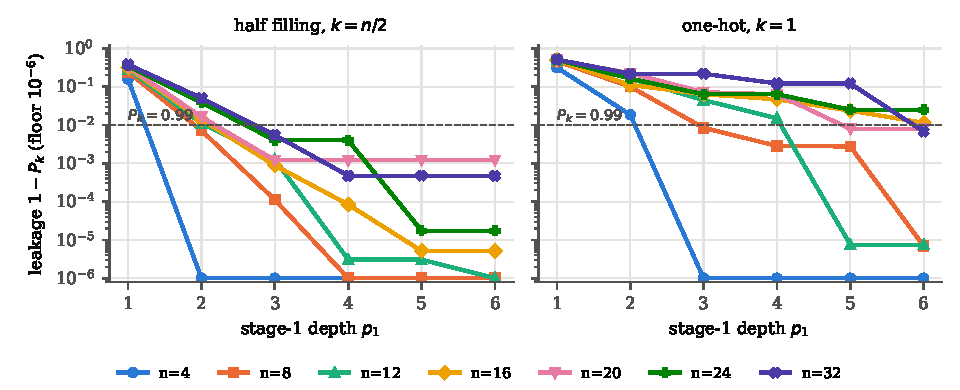
\includegraphics[width=\linewidth]{stage1_table.pdf}
\caption{Leakage $1-P_k$ of the tabulated stage-1 states versus depth. Left: half filling; right: one-hot.}
\label{fig:stage1}
\end{figure}
Table~\ref{tab:stage1} and Fig.~\ref{fig:stage1} list the stage-1 states for group sizes up to $n=32$.
For half filling, three layers reach $P_k\ge0.9945$ for every tested size ($n=4$--$32$; the lowest value is $0.99454$ at $n=32$), and four layers reach $P_k\ge0.996$; within the tested range, three layers are an observed sufficient depth independent of $n$.
For one-hot groups the smallest depth found reaching $P_k\ge0.99$ grows: three layers up to $n=8$, four for $n=10$, five for $n=12$ and $n=20$, and six for $n=32$, while $n=16$ and $n=24$ stay at $0.989$ and $0.975$ at $p_1=6$. These are values found by local optimization, not lower limits on the depth.
Plateaus such as $n=24$, $k=1$ at $p_1=3$ and $4$ show that the optimizer stopped in a local optimum, so these entries are lower bounds.
For comparison, the entangling-free biased product state has $P_k\approx0.37$--$0.42\approx1/e$ for $k=1$ and $\binom{n}{n/2}2^{-n}$ ($0.14$--$0.27$ for $n\ge8$) for half filling.

\subsection{Cardinality-constrained portfolios}
\begin{figure}[t]\centering
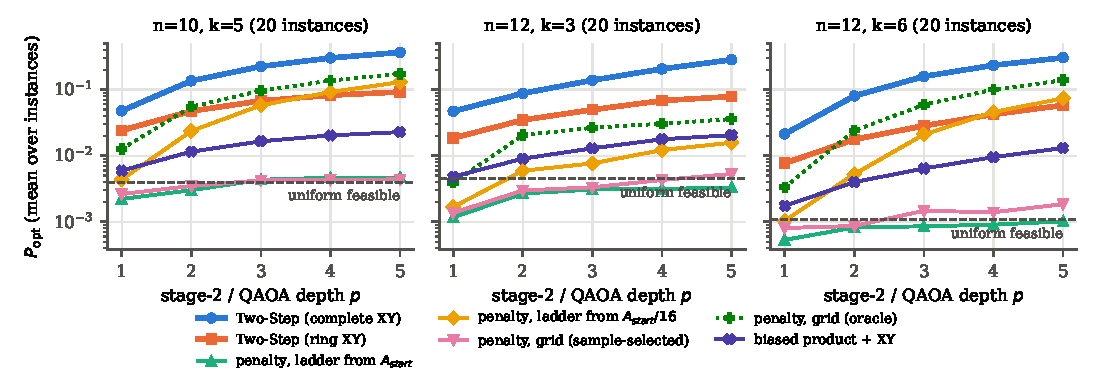
\includegraphics[width=\linewidth]{portfolio.pdf}
\caption{Mean optimum probability versus depth for portfolio problems. The Dicke-initialized ansatz agrees with ring-mixer Two-Step up to the factor $P_{\mathcal G}$ (apart from rare differences in the local optimum reached by training) and is not drawn.}
\label{fig:portfolio}
\end{figure}
\begin{table}[t]\centering\small
\caption{Portfolio problems, Two-Step with the ring XY mixer: paired ratio $P_{\rm opt}^{\rm Two\text{-}Step}/P_{\rm opt}^{\rm baseline}$ per instance at the same depth $p$; median with 95\% bootstrap interval of the median, and the number of instances in which Two-Step is better. Budgets: ladders as used (all stopped at their first rung), grids five weights, post-selected methods with overhead $1/P_k$. The biased-product baseline uses the ring XY mixer.}
\label{tab:portfolio}
\resizebox{\linewidth}{!}{\begin{tabular}{llccc}\toprule
$(n,k)$ & baseline & $p=1$ & $p=3$ & $p=5$\\\midrule
(10,5) & uniform feasible & 5.41 [3.46, 7.03] (20/20) & 14.12 [7.96, 18.90] (19/20) & 16.26 [9.53, 28.91] (19/20)\\
(10,5) & penalty, ladder from $A_{\rm start}$ & 9.50 [6.21, 12.66] (20/20) & 12.86 [7.22, 17.73] (19/20) & 14.22 [8.21, 24.41] (19/20)\\
(10,5) & penalty, ladder from $A_{\rm start}/16$ & 5.28 [3.49, 7.10] (20/20) & 1.21 [0.60, 1.73] (11/20) & 0.67 [0.23, 0.81] (5/20)\\
(10,5) & penalty, grid (sample-selected) & 7.50 [5.97, 11.95] (20/20) & 13.23 [7.19, 17.78] (19/20) & 15.26 [8.72, 25.94] (19/20)\\
(10,5) & penalty, grid (oracle-selected) & 1.69 [1.17, 2.29] (17/20) & 0.70 [0.33, 1.20] (7/20) & 0.52 [0.18, 0.82] (4/20)\\
(10,5) & biased product + XY & 4.06 [4.06, 4.06] (20/20) & 4.06 [4.06, 4.06] (20/20) & 4.06 [4.06, 4.06] (20/20)\\
\midrule
(12,3) & uniform feasible & 3.55 [3.28, 4.69] (20/20) & 8.12 [6.58, 11.29] (20/20) & 15.03 [6.43, 22.41] (19/20)\\
(12,3) & penalty, ladder from $A_{\rm start}$ & 13.70 [12.68, 18.20] (20/20) & 12.04 [9.65, 16.70] (20/20) & 20.68 [8.90, 31.13] (19/20)\\
(12,3) & penalty, ladder from $A_{\rm start}/16$ & 9.72 [8.48, 12.79] (20/20) & 5.13 [3.74, 7.46] (19/20) & 4.68 [1.91, 5.99] (17/20)\\
(12,3) & penalty, grid (sample-selected) & 12.81 [10.24, 17.76] (20/20) & 11.06 [9.14, 16.94] (20/20) & 13.92 [5.36, 24.75] (19/20)\\
(12,3) & penalty, grid (oracle-selected) & 5.27 [3.92, 5.85] (20/20) & 2.21 [1.18, 2.81] (15/20) & 1.62 [0.79, 3.21] (12/20)\\
(12,3) & biased product + XY & 3.84 [3.82, 3.84] (20/20) & 3.84 [3.84, 3.84] (20/20) & 3.84 [3.84, 3.84] (20/20)\\
\midrule
(12,6) & uniform feasible & 5.62 [3.94, 8.43] (20/20) & 15.89 [12.22, 30.23] (20/20) & 36.11 [8.78, 71.07] (20/20)\\
(12,6) & penalty, ladder from $A_{\rm start}$ & 11.36 [7.99, 17.11] (20/20) & 20.10 [15.40, 38.47] (20/20) & 39.13 [9.72, 73.92] (20/20)\\
(12,6) & penalty, ladder from $A_{\rm start}/16$ & 5.78 [3.98, 9.10] (20/20) & 1.19 [0.74, 2.63] (13/20) & 0.94 [0.30, 1.62] (8/20)\\
(12,6) & penalty, grid (sample-selected) & 8.04 [5.22, 14.29] (20/20) & 17.49 [8.92, 37.49] (20/20) & 24.92 [7.93, 41.95] (19/20)\\
(12,6) & penalty, grid (oracle-selected) & 1.79 [1.42, 2.69] (18/20) & 0.51 [0.41, 0.80] (6/20) & 0.36 [0.19, 0.55] (3/20)\\
(12,6) & biased product + XY & 4.43 [4.42, 4.43] (20/20) & 4.43 [4.43, 4.43] (20/20) & 4.43 [4.43, 4.43] (20/20)\\
\bottomrule\end{tabular}}\end{table}

We use cardinality-constrained portfolios, $\min_x\,\tfrac12x^\top\Sigma x-\mu^\top x$ subject to $\sum_ix_i=k$, with $\Sigma=AA^\top/n$ for a standard normal $A$ and $\mu_i\sim U(0,1)$, for $(n,k)=(10,5)$, $(12,3)$ and $(12,6)$ and 20 random instances each (Fig.~\ref{fig:portfolio}, Table~\ref{tab:portfolio}).
Three points stand out.

\emph{At shallow depth Two-Step QAOA has the higher optimum probability.} At $p=1$ the median paired ratio is $3.5$--$5.6$ against uniform feasible sampling and $5.3$--$13.7$ against the ladder- and sample-selected penalty rules, in all 20 instances of every size; the oracle-tuned grid with five times the budget is behind by a median factor $1.7$--$5.3$ (Two-Step is better in 17, 20 and 18 of 20 instances).
The ladder that starts from the formulation code's $A_{\rm start}$ always stops at its first rung, because a large weight produces feasible samples immediately; its mean optimum probability then stays at or below the level of uniform sampling ($0.3$--$1.2$ times) at all depths. Selecting the weight from the grid by the sampled answers does not help either: it picks $A\ge0.3\sigma$ in 281 of the 300 (instance, depth) cases, where the optimum probability is low, presumably because batches from such weights already contain good feasible answers.

\emph{With the ring mixer, a small penalty weight catches up at larger depth for half filling.} The ladder started from $A_{\rm start}/16$ (which also stopped at its first rung) improves quickly with depth: at $p=5$ it beats ring-mixer Two-Step in 15 of 20 instances for $(10,5)$ and 12 of 20 for $(12,6)$ (median ratios $0.67$ and $0.94$), at the same training budget, while it remains behind for $(12,3)$ (median $4.7$, 17 of 20). The oracle-tuned grid is better than ring-mixer Two-Step from $p=3$ on for half filling. A small weight leaves roughly half of the samples infeasible ($P_{\rm feas}\approx0.5$--$0.6$), but the $X$ mixer can move through infeasible strings, which the ring XY mixer cannot.

\emph{With the complete-graph mixer, Two-Step is ahead at every depth.} Replacing the ring by all pairs of the group (the same number of two-qubit terms per layer as the cost layer) raises the optimum probability of Two-Step by a median factor $1.4$--$6.3$ (Table~\ref{tab:portfolio_complete}). In median it is then better than every baseline at every depth, including the oracle-tuned grid with five times the budget (median ratios $2.2$--$9.7$ at $p\ge3$, in 18--20 of 20 instances), and better than the small-weight ladder by median factors $2.9$--$17$ at $p=5$. The crossover in the previous paragraph was therefore a limitation of the ring mixer, not of the hard-constraint approach.
\begin{table}[t]\centering\small
\caption{Portfolio problems, Two-Step with the complete-graph XY mixer: paired ratio $P_{\rm opt}^{\rm Two\text{-}Step}/P_{\rm opt}^{\rm baseline}$ per instance at the same depth $p$; median with 95\% bootstrap interval of the median, and the number of instances in which Two-Step is better. Budgets: ladders as used (all stopped at their first rung), grids five weights, post-selected methods with overhead $1/P_k$. The biased-product baseline uses the ring XY mixer.}
\label{tab:portfolio_complete}
\resizebox{\linewidth}{!}{\begin{tabular}{llccc}\toprule
$(n,k)$ & baseline & $p=1$ & $p=3$ & $p=5$\\\midrule
(10,5) & uniform feasible & 10.96 [9.90, 15.72] (19/20) & 50.66 [36.80, 65.18] (20/20) & 87.42 [68.35, 102.58] (20/20)\\
(10,5) & penalty, ladder from $A_{\rm start}$ & 19.25 [17.96, 27.81] (20/20) & 47.12 [32.03, 58.16] (20/20) & 73.32 [59.48, 90.70] (20/20)\\
(10,5) & penalty, ladder from $A_{\rm start}/16$ & 10.97 [8.33, 14.20] (20/20) & 3.68 [3.37, 4.52] (20/20) & 2.87 [2.43, 3.15] (20/20)\\
(10,5) & penalty, grid (sample-selected) & 18.63 [13.82, 25.62] (20/20) & 47.01 [32.17, 64.11] (20/20) & 79.75 [59.32, 96.82] (20/20)\\
(10,5) & penalty, grid (oracle-selected) & 3.60 [2.88, 4.48] (19/20) & 2.21 [1.91, 3.04] (20/20) & 2.24 [1.78, 2.77] (20/20)\\
(10,5) & biased product + XY & 9.15 [5.98, 12.89] (20/20) & 16.65 [10.48, 25.19] (20/20) & 18.34 [12.85, 39.68] (20/20)\\
(10,5) & Two-Step (ring XY) & 2.25 [1.48, 3.18] (17/20) & 4.10 [2.42, 6.20] (19/20) & 4.87 [3.16, 9.77] (19/20)\\
\midrule
(12,3) & uniform feasible & 6.25 [2.31, 7.25] (15/20) & 29.24 [21.55, 36.95] (19/20) & 56.28 [46.33, 66.70] (20/20)\\
(12,3) & penalty, ladder from $A_{\rm start}$ & 24.56 [9.04, 28.73] (17/20) & 42.69 [31.59, 54.51] (19/20) & 75.55 [63.70, 93.84] (20/20)\\
(12,3) & penalty, ladder from $A_{\rm start}/16$ & 17.88 [6.69, 19.19] (16/20) & 17.57 [13.11, 22.09] (18/20) & 17.22 [12.20, 24.27] (19/20)\\
(12,3) & penalty, grid (sample-selected) & 20.13 [8.78, 28.14] (17/20) & 41.68 [30.27, 52.26] (19/20) & 59.67 [44.79, 77.15] (20/20)\\
(12,3) & penalty, grid (oracle-selected) & 7.22 [2.69, 9.56] (15/20) & 6.86 [3.80, 10.50] (18/20) & 9.68 [5.94, 10.56] (19/20)\\
(12,3) & biased product + XY & 5.20 [2.51, 7.15] (15/20) & 9.88 [5.95, 22.05] (19/20) & 17.86 [11.73, 28.25] (20/20)\\
(12,3) & Two-Step (ring XY) & 1.36 [0.65, 1.86] (13/20) & 2.57 [1.55, 5.75] (17/20) & 4.65 [3.06, 7.36] (18/20)\\
\midrule
(12,6) & uniform feasible & 17.49 [13.49, 24.95] (19/20) & 127.53 [84.99, 162.24] (20/20) & 269.61 [163.83, 348.12] (20/20)\\
(12,6) & penalty, ladder from $A_{\rm start}$ & 36.15 [27.19, 51.67] (20/20) & 158.90 [108.86, 205.59] (20/20) & 287.54 [177.34, 370.46] (20/20)\\
(12,6) & penalty, ladder from $A_{\rm start}/16$ & 18.61 [14.74, 24.39] (19/20) & 7.40 [6.04, 8.83] (20/20) & 4.72 [3.63, 7.22] (20/20)\\
(12,6) & penalty, grid (sample-selected) & 24.81 [21.48, 32.33] (20/20) & 152.99 [84.33, 198.96] (20/20) & 167.66 [112.08, 266.49] (20/20)\\
(12,6) & penalty, grid (oracle-selected) & 6.09 [5.22, 7.61] (19/20) & 2.70 [2.29, 4.91] (20/20) & 2.50 [2.19, 2.80] (20/20)\\
(12,6) & biased product + XY & 13.19 [9.24, 21.75] (19/20) & 24.64 [19.03, 49.09] (20/20) & 28.02 [19.01, 51.85] (20/20)\\
(12,6) & Two-Step (ring XY) & 3.00 [2.06, 4.92] (18/20) & 5.56 [4.30, 11.09] (20/20) & 6.33 [4.29, 11.71] (19/20)\\
\bottomrule\end{tabular}}\end{table}


Two further observations confirm the theory. The Corollary predicts $P_{\rm opt}^{\rm Two\text{-}Step}=P_{\mathcal G}P_{\rm opt}^{\rm Dicke}$ for identical stage-2 angles, and, applied to the biased product state (whose weight-$k$ component is also the Dicke state), a fixed ratio $P_{\mathcal G}/P_k^{\rm product}=4.06$, $3.84$ and $4.43$ for the three sizes. Since the three methods are trained from independent starts, the angles need not coincide; in practice both relations hold to within $0.1\%$ in 84--89\% of the (instance, depth) pairs, and the remaining pairs deviate by at most $3\%$ except one pair with $34\%$, where training reached a different local optimum. The median ratios for the ring-mixer biased product state in Table~\ref{tab:portfolio} equal the predicted values.

\subsection{Detecting constraints}
\begin{table}[t]\centering\small
\caption{Detecting k-hot penalties from QUBO matrices of 168 instances of 29 formulations. Truth: the constraints passed to the penalty builders. Final detections are counted correct only if both the support and $k$ match. Totals: 1179 constraints, 562 detections, 487 correct (precision 0.87, recall 0.41); candidate supports before the $k$ fit: 20541, of which 983 match a true support.}
\label{tab:detect}
\begin{tabular}{lrrrr}\toprule
formulation & constraints & detections & correct & wrong\\\midrule
assignment & 72 & 71 & 71 & 0\\
bin-packing & 51 & 0 & 0 & 0\\
clique & 0 & 14 & 0 & 14\\
clustering & 60 & 44 & 44 & 0\\
coloring & 51 & 51 & 51 & 0\\
community & 60 & 60 & 60 & 0\\
facility & 42 & 0 & 0 & 0\\
feature-selection & 6 & 0 & 0 & 0\\
flowshop & 48 & 42 & 42 & 0\\
graph-partition & 6 & 2 & 0 & 2\\
jobshop & 46 & 42 & 42 & 0\\
knapsack & 0 & 2 & 0 & 2\\
maxcut & 0 & 15 & 0 & 15\\
maze & 0 & 7 & 0 & 7\\
mis & 0 & 5 & 0 & 5\\
number-partition & 0 & 7 & 0 & 7\\
portfolio & 6 & 0 & 0 & 0\\
portfolio-constrained & 6 & 0 & 0 & 0\\
production & 30 & 0 & 0 & 0\\
qap & 60 & 60 & 60 & 0\\
qubo & 0 & 1 & 0 & 1\\
set-cover & 0 & 3 & 0 & 3\\
shift & 336 & 0 & 0 & 0\\
sudoku & 71 & 8 & 3 & 5\\
timetable & 30 & 24 & 24 & 0\\
tsp & 90 & 90 & 90 & 0\\
vertex-cover & 0 & 8 & 0 & 8\\
vrp & 108 & 6 & 0 & 6\\
\bottomrule\end{tabular}\end{table}

We applied the detector of Sec.~\ref{sec:detect} to the QUBO matrices produced by the penalty builders of a library of 29 formulations (Table~\ref{tab:detect}); the truth is the list of constraints those builders were given.
Of $562$ detections, $487$ are correct in both support and $k$ (precision $0.87$), but only $41\%$ of the $1179$ constraints are found.
The support is usually recognized (candidate supports cover $983$ true supports), and the losses are where the Remark of Sec.~\ref{sec:theory} predicts them: when the cost has large linear terms on a group (facility location, shift scheduling, vehicle routing), $k$ is misread; when the cost adds to the couplings inside the group (portfolio) or inequality penalties dominate (bin packing, production), the support is missed; and unconstrained problems with uniform couplings (MaxCut, vertex cover) produce false constraints.
The detector is therefore usable as a suggestion for formulations whose penalties dominate uniformly (assignment, coloring, QAP, TSP), but the constraints should be passed explicitly.

\subsection{Several groups: coloring and permutation problems}
\begin{table}[t]\centering\small
\caption{Problems with several one-hot groups (mean over instances, depth $p=5$, ring XY mixer). ``Hard'' rows: the one-hot groups chosen by the formulation code are hardened with XY mixers; for coloring these are all constraints, for the permutation problems only the rows (columns remain penalties). $P_{\rm opt|feas}$ is the optimum probability among feasible samples. Penalty weights follow the formulation code's ladder.}
\label{tab:multi}
\begin{tabular}{lrrlccc}\toprule
problem & qubits & inst. & method & $P_{\rm feas}$ & $P_{\rm opt}$ & $P_{\rm opt|feas}$\\\midrule
assignment 4 & 16 & 5 & uniform feasible & 1.000 & 0.0417 & 0.0417\\
assignment 4 & 16 & 5 & penalty QAOA & 0.063 & 0.0055 & 0.0885\\
assignment 4 & 16 & 5 & Two-Step (rows hard) & 0.614 & 0.1140 & 0.1850\\
\midrule
graph 3-coloring (dense) 4 & 12 & 10 & uniform feasible & 1.000 & 0.3111 & 0.3111\\
graph 3-coloring (dense) 4 & 12 & 10 & penalty QAOA & 0.972 & 0.4043 & 0.4174\\
graph 3-coloring (dense) 4 & 12 & 10 & Two-Step (all hard) & 1.000 & 0.9861 & 0.9861\\
\midrule
graph 3-coloring (dense) 5 & 15 & 10 & uniform feasible & 1.000 & 0.1185 & 0.1185\\
graph 3-coloring (dense) 5 & 15 & 10 & penalty QAOA & 0.788 & 0.1290 & 0.1761\\
graph 3-coloring (dense) 5 & 15 & 10 & Two-Step (all hard) & 1.000 & 0.9302 & 0.9302\\
\midrule
QAP 4 & 16 & 5 & uniform feasible & 1.000 & 0.0583 & 0.0583\\
QAP 4 & 16 & 5 & penalty QAOA & 0.057 & 0.0044 & 0.0800\\
QAP 4 & 16 & 5 & Two-Step (rows hard) & 0.780 & 0.0633 & 0.0822\\
\midrule
TSP 4 & 16 & 5 & uniform feasible & 1.000 & 0.3333 & 0.3333\\
TSP 4 & 16 & 5 & penalty QAOA & 0.025 & 0.0096 & 0.3876\\
TSP 4 & 16 & 5 & Two-Step (rows hard) & 0.848 & 0.3298 & 0.3890\\
\bottomrule\end{tabular}\end{table}

Table~\ref{tab:multi} uses problems from the same formulation library, with the library's own penalty ladders; Two-Step uses the ring mixer here.
\emph{Graph 3-coloring} (dense random graphs with edge probability $0.7$; minimizing the number of monochromatic edges) has one one-hot group per vertex, all disjoint, so every constraint is hardened and no penalty weight remains.
Two-Step then finds an optimal coloring with probability $0.93$ (5 vertices, 15 qubits) and $0.99$ (4 vertices, 12 qubits) at $p=5$, against $0.13$ and $0.40$ for penalty QAOA and $0.12$ and $0.31$ for uniform sampling. (The 12-qubit value is close to saturation, so the 15-qubit case is the informative one.)
\emph{Permutation problems} (assignment, QAP, TSP on $4\times4$ variables) have one-hot rows and columns; only the rows are hardened and the columns remain penalties. Hardening raises $P_{\rm feas}$ from $0.025$--$0.063$ to $0.61$--$0.85$ and improves the optimum probability over penalty QAOA by a factor $14$--$34$. Against uniform sampling of permutations it is better for assignment ($0.114$ versus $0.042$) and on par for QAP ($0.063$ versus $0.058$) and TSP ($0.330$ versus $0.333$); the quality inside the feasible set is only modestly above uniform. With only 24 feasible permutations (and 8 optimal tours for TSP) these instances are small, and the comparison with uniform sampling is the relevant one.
